Parmi les trois étapes constitutives de la phase de décomposition,
seule la décomposition des \emph{relations de localisation} nécessite
le développement d'une méthode spécifique. En effet, les étapes de
décomposition de ensemble des \emph{indices de localisation} et des
\emph{objets de référence indéfinis} ne font qu'expliciter un
découpage présent dès la saisie. Ces deux opérations ne nécessitent
donc pas l'apport de connaissances supplémentaires, contrairement à la
décomposition des \emph{relations de localisation.}

En effet, les \emph{principes de décomposition} et de
\texttt{intégration contexte métier} s'opposent en partie. Si la
décomposition permet de faciliter la \emph{spatialisation} des
\emph{indices de localisation} en permettant de manipuler des concepts
précis et en minimisant les redondances, elle implique également de
travailler à l'aide de \emph{relations de localisation} (atomiques)
\emph{ad hoc,} qui ne sont pas destinées à être manipulées directement
par l'utilisateur. Il est donc inenvisageable de demander à
l'utilisateur de saisir des \emph{relations de localisation
  atomiques,} qui ne sont pas prévues pour. C'est pourquoi nous
proposons d'automatiser cette étape.

\subsection{La décomposition des \emph{relations de localisation}}

Nous avons précédemment abordé la décomposition des \emph{relations de
  localisation} en la présentant comme le processus permettant de
passer d'une \emph{relation de localisation} à un ensemble de
\emph{relations de localisations atomiques} liées par des conjonctions
et auxquelles est apposée une méthode de \emph{spatialisation,}
permettant de construire la \emph{zone de localisation compatible}
correspondant à la \emph{relation de localisation atomique} pour un
\emph{objet de référence} donné.

Cette définition n'offre cependant pas un aperçu complet des
situations possibles.

On peut également imaginer un cas où une \emph{relation de
  localisation} se décompose en plusieurs \emph{relations de
  localisation,} elles-mêmes décomposables. La décomposition est alors
récursive.





La difficulté de la décomposition des relations de localisation dépend
principalement d'un seul choix, celui de la définition ---~ou non~---
de décompositions concurrentes pour la même \emph{relation de
  localisation.} Dans le cas où chaque relation de localisation n'a
qu'une décomposition possible, il suffit de l'appliquer pour
construire de nouveaux indices de localisation à partir de l'unique
décomposition de la relation de localisation. Dans le cas contraire,
il est nécessaire de choisi quelle décomposition appliquer parmi un
panel de possibles, ce qui impose de disposer d'une heuristique et de
données permettant de justifier ce choix. Si elles sont éminemment
plus complexes à mettre en place, de telles décompositions permettent
d’adapter la spatialisation au contexte.




L'automatisation de la décomposition des \emph{relations de
  localisation} nécessite la définition à priori d'un ensemble de
règles, définissant la manière dont les différentes \emph{relations de
  localisation} se décomposent (cf. présentation du \emph{principe de
  modélisation explicite des connaissances}, \autoref{chap:04}). 



Nous avons choisi de formaliser ces décomposition
au sein d'une ontologie, créée pour l'occasion.

La décomposition des relations de localisation nécessite donc deux
étapes. La première est la lecture des règles de décomposition, la
seconde est leur application.

\tdi{le secouriste à un choix limité}

Pour 

\tdi{Bivalence décomposition-relations de localisation}





\tdi{Possibilité de faire des négations}

Il est également envisageable de permettre l'utilisation de négations
de relations de localisation atomiques. Ainsi on pourra utiliser


\tdi{Pas de limitations nombre de décompositions}


L'application des règles de décomposition n'est pas particulièrement
déclicate, 


\begin{figure}
  \centering
  \missingfigure{}
  \caption{Illustration du processus de décomposition des relations de
  localisation}
  \label{fig:logique_dec}
\end{figure}

\subsection{Vers la définition d'une ontologie des règles de
  décomposition des \emph{relations de localisation}}

Nous avons choisi de formaliser les règles de décomposition des
\emph{relations de localisation} à l'aide d'une ontologie de
décomposition. Cette dernière doit contenir, a minima, trois types
d'informations :
%
\begin{enumerate*}[label=(\alph*)]
\item \emph{les relations de localisation} à décomposer,
\item les \emph{relations de localisation atomiques} qui les
  décomposent et
\item les \emph{relations de décomposition} formalisant la
  décomposition d'une \emph{relation de localisation} en plusieurs
  \emph{relations de localisations atomiques}
  (\autoref{fig:onto_min_struct}).
\end{enumerate*}
%
L'ensemble des \emph{relations de localisation} définies dans
l'ontologie forme un vocabulaire contrôlé, qui peut être utilisé dans
plusieurs aspects du projet Choucas. 

\tdi{parler de l'utilisation de l'ontologie dans d'autres domaines
  (lots 4 et 2)}


permettant à l'utilisateur
de saisir les \emph{indices de localisation}. La décomposition de ces
relations ne lui est pas connue. Le travail de décomposition ne
consiste alors qu'à appliquer la règle de décomposition ---~définie
dans l'ontologie~--- correspondant à la \emph{relation de
  localisation} saisie.

\begin{figure}
  \centering
  \usetikzlibrary{patterns}
\usetikzlibrary{fadings}
\usetikzlibrary{external}
\usetikzlibrary{calc}
\usetikzlibrary{positioning}
\usepgfplotslibrary{colormaps}
\usetikzlibrary{arrows}
\usetikzlibrary{matrix}

\usetikzlibrary{trees}


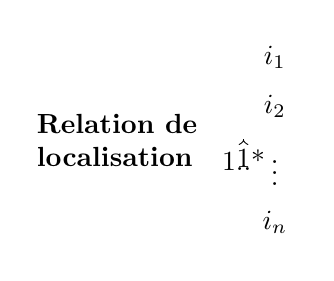
\begin{tikzpicture}
  \tikzset{
    acc/.style={decorate,decoration={brace,raise=0cm,amplitude=.1cm}},
    accm/.style={acc,decoration={mirror}},
    acc3/.style={acc,decoration={amplitude=.2cm}},
    acc3m/.style={acc3,decoration={mirror}}
  }
  
%% Matrices
\node[font=\bfseries, baseline, text width=2.5cm] (I) at (0,0) {Relation de localisation};

\matrix [matrix of math nodes,row sep=0.1cm,column sep=0.1cm,
anchor=west, nodes={anchor=base, baseline}] (is) at (I.east)
{i_1\\i_2\\\vdots{}\\i_n\\};

\draw[->, black] (I.east) -- (is.west) node[pos=0,below] {1} node[pos=1,below]{1..*};

\end{tikzpicture} 
  \caption[Structure générale d'une ontologie de
  décomposition]{Concepts et relations nécessaires à la définition
    d'une ontologie permettant de décomposer une \emph{relation de
      localisation} ($rl_i$) en un ensemble de \emph{relations de
      localisation atomiques} ($rla_i$).}
  \label{fig:onto_min_struct}
\end{figure}

\tdi{Parler du fait que la décomposition des rl puisse être
  récursive.}

Comme nous l'expliquions lors de la présentation de la phase de
décomposition, chacune des étapes de cette phase consiste à créer un
nouvel \emph{indice de localisation.} Conformément au \emph{principe
  de modélisation autonome,} chaque \emph{indice de localisation}
traité peut être décomposé de manière indépendante.

Comme le montre la \autoref{fig:onto_min_struct}, plusieurs
configurations de décompositions sont envisageables. La première
d'entre-elles ---~la plus courante~--- est la décomposition d'une
\emph{relation de localisation} en plusieurs \emph{relations de
  localisation atomiques} (\eg \(rk_1\) et \(rl_3\),
cf. \autoref{fig:onto_min_struct}).
%
Ces dernières peuvent partager une \emph{relation de localisation
  atomique} (\eg \(rk_2\) et \(rl_3\) dont la décomposition contient
\(rla_3\)), ce qui est souhaité par le \emph{principe de
  décomposition.}
%
Dans certaines configurations (\eg \(rl_2\)), on ne peut pas
identifier de décomposition satisfaisante pour une \emph{relation de
  localisation.} La \emph{relation de localisation} n'est alors que
l'alias d'une \emph{relation de localisation atomique.} Dans ce cas il
n'est pas nécessaire de définir (contrairement a ce qui a été fait
pour l'exemple de la \autoref{fig:onto_min_struct}), une
\emph{relation de localisation} et une \emph{relation de localisation
  atomique,} on peut simplement définir la seconde et la présenter à
l'utilisateur comme une \emph{relation de localisation non atomique.}

Pour construire la base des relations de localisation, des relations
de localisation atomiques et des relations de décomposition en tre ces
deux ensembles nous avons adopté, conformément au principe
d'intégration dans le contexte métier, une démarche centrée sur le
besoin de l'utilisateur, \ie fondée sur la définition préalable des
\emph{relations de localisation.} Ainsi les relations de localisation
atomiques et les relations de décomposition sont définies
ultérieurement, par rapport aux relations de localisation et non
l'inverse, ce qui pourrait conduite à la définition de concepts
inadaptés à notre contexte applicatif.  En procédant de la sorte nous
garantissions que les concepts mis à disposition des utilisateurs
correspondent à la réalité du contexte applicatif. Pour mettre en
place cette démarche, il est nécessaire d'identifier les
\emph{relations de localisations} utilisées dans notre contexte et les
spécificités de leur usage.

\tdi{liens avec Bateman}

%%% Local Variables:
%%% mode: latex
%%% TeX-master: "../../../../main"
%%% End:
